\chapter{Background}
\label{cha:background}

\begin{comment}
Chapter 2: Background and literature survey
This chapter should give essential background information with references to published material in research papers, books, URLs, magazine articles and even newspapers. Expand on any references to other work that have been mentioned in Chapter 1. Refer to the notes on references (below) for the preferred way of referencing publications. The reader, stimulated by the presentation of ideas in this section, may be led to consult some or all of the referenced publications. This section will be useful for any student in a subsequent year who wishes to take the project further.
\end{comment}

\section{Financial Management}
There are several other applications that implement money management features found in this project, most notably Lloyds TSB Money Manager, the first personal money management application provided by a UK bank and Mint.com a US only personal finance service \parencite{lloyds2014moneymanager, mint2014whatismint}.

\subsection{Lloyds Money Manager}
The service is available to Lloyds TSB current account holders as part of their online banking and it's features revolve around documenting historical spending.

The key features are as follows \parencite{lloyds2014money}:
\begin{itemize}
\item Categorising spending
\item Creating spending plans per category
%\item View dates money came in and out in a calendar
\item Viewing money spent per category
\item Track progress of budget targets
\end{itemize}

\begin{figure}[h]
    \centering
    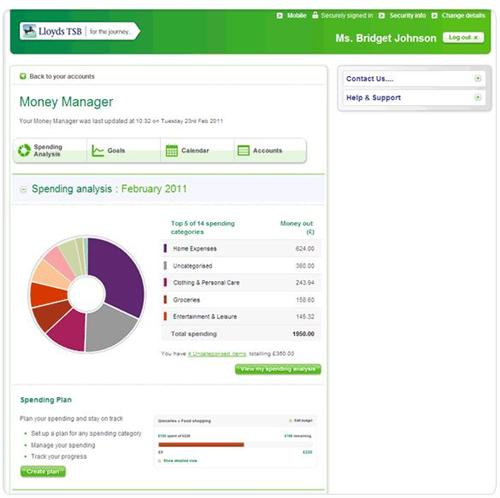
\includegraphics{background/moneymanagerchart}
    \caption{Spending Analysis on Money Manager \parencite{lloyds2014money}}
    \label{fig:moneymanager}
\end{figure}

Customer reviews of the product highlight how useful the spending analysis screen, which includes a breakdown of spending in each category is as well as the spending calendar, which displays money spent in a calendar format. The reviews, however also suggest some shortcomings, noting that changes to categories are not reflected immediately and that it's unable to override the category for a single spend (e.g. food bought at a petrol station is placed in the Car category) \cite{moneywatch2011lloyds}.

A key advantage of the money manager is that Lloyds already have all their customer data, so there is no data entry or upload step, which could potentially be confusing users.

\subsection{Mint.com}
Mint.com offers very similar features to LLoyds but it limited to the US. However, Mint automatically logs into the users online bank account and downloads their statements authenticating with their banking username and password, it is believed that this feature relies on API's at each bank which Intuit (the company behind Mint) have negotiated access to individually, though Intuit provide no information on this \cite{stackoverflow2012bankingapi, stackoverflow2012bankingapi2}. Although this feature is clearly useful and saves time for the users, it does make Mint responsible for storing their customers Internet banking passwords and presumably involves fee payments to the banks providing these API's. For these reasons was decided that automatic statement downloading is outside of the scope of this project.

\plan{More detail on what mint/lloyds do?}

\subsection{Mobile Apps}
Mobile applications or `apps' as they are commonly known have seen a surge in popularity since the release of startphones and are a common target for small pieces of software, such as financial organisation.

The three most popular iPhone personal financial applications \cite{itunes2013topapps}, at the time of planning the project, all offered features very similar to those found in the Lloyds Money Manager and Mint. The most popular features being grouping money by category and graphs of spending history. However, they all had the same drawback, the user had to manually enter all of their transactions and set categories for them, which appears time consuming and error prone, particularly on a mobile app \cite{spendee2014spendee,budgt2013budgt,bluetags2014pocket}.

The increase of mobile usage however should be considered when planning the features of the project, with the project ensuring mobile compatibility.

\section{Prediction}

\todo[inline]{Make this make sense}
Predicting future expenditure given previous history is notoriously hard. There have been several different approaches to this in the past in the context of personal finance, but by opening up to other finance predictions such as those on the stock market, there is a lot more research.
\todo[inline]{Finish this}

%\plan{Ways other people try to predict the future expenditure (in stocks etc...)}

There are various approaches to making predictions of financial spending, each with their own advantages and disadvantages. Predicting future transactions before they occur is technically similar to the work done by investors on the stock market, where the objective is to predict whether the value of a stock will fall or increase in order to make buy/sell decisions.

\plan{I need at least two more papers, preferably some using Markov Chains}


Preifer and Carraway demonstrated that Markov Chain Models can be used to model customer relationships with a business and predict the expected value of a marketing engagement with an individual customer. By creating a transition matrix of a particular customer transitioning from not spending to spending and visa versa over five periods\footnote{An `illustration' assuming a customer will never return after 5 months of not spending}, they were able to estimate the likely-hood of a spend occurring in a given period, Fig. \ref{fig:preifermarkovchain} shows a graphical representation of the model that was produced, the states represent the five periods, where $p_{i}$ is the probability of the transition occurring during period $i$ \cite{pfeifer2000modeling}.
% 
The paper is able to calculate the expected loan to value ratio (LTV) for the customer over the periods, by taking a matrix costs and gains associated with a purchase in each period and multiplying that by the probability of a purchase occurring taken from the transition matrix. This gives the expected present value for each period, which can be used to decide when to end a relationship with a customer (preventing the costs).
%
They demonstrate applying Markov Chain Models to a larger dataset, calculating the optimal policy for ending relationships with customers depending on varying costs concluding that the use of MCM's is an effective way of making customer relationship decisions. However, this paper assumes the company performing these predictions already knows how much money a customer will spent during each interactions and is focussed around calculating the probability of a spend occurring. An implementation applied to the personal spending space will require a way to predict the value of the future transaction.
\question{Mention what HMM's are here?}

\begin{figure}[h]
    \centering
    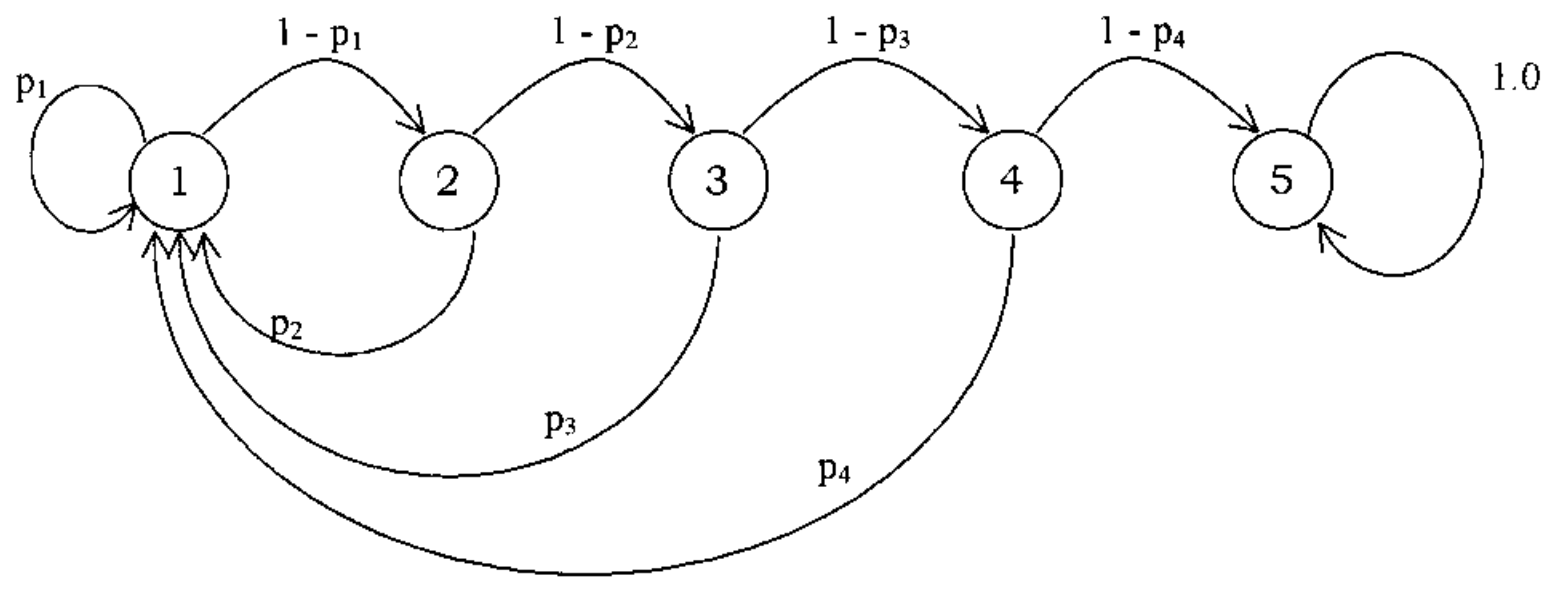
\includegraphics[width=\textwidth]{background/markovchain}
    \caption{Markov Chain Model for a particular customer over five periods \parencite[Fig. 1]{pfeifer2000modeling}}
    \label{fig:preifermarkovchain}
\end{figure}

Research by Singh et al., from the Massachusetts Institute of Technology, studied the spending behaviour of 52 adults and investigated the impact of social interactions, including text messages, phone calls and face-to-face meetings, on the participants spending in order to predict their spending behaviour. Using a Na\"{i}ve Bayes classifier and selecting a subset of their available features using an Information Gain approach, choosing those with most relevance to each classification task, they were able to correctly classify whether the participant would overspend, explore a diverse range of businesses and remain loyal to a business with 72\% overall accuracy. They concluded that social factors, were better ``predictors of spending behaviour'' than personality traits, which had been previously studied \parencite{singh2013spendingbehaviour}.
%
Although this paper did not study the affects of the participants previous transactions on spending, they were able to predict the users spending behaviour, highlighting that factors other than the transaction history may be of importance when trying to predict a users future outflow. However, the paper does not attempt to make a prediction of the amount spent or how many transactions occur.

Smoothing is typically applied to financial market data, for example the value of a particular stock on the FTSE 100. The most common techniques are simple, weighted and exponential moving averages, which all reduce the noise found in the data potentially revealing an orderly process, by removing outliers found in the data. The result of this effect can be seen in Fig \ref{fig:dashweightedaverages} \parencite{dash2012movingaverages}.

\begin{figure}[h]
    \centering
    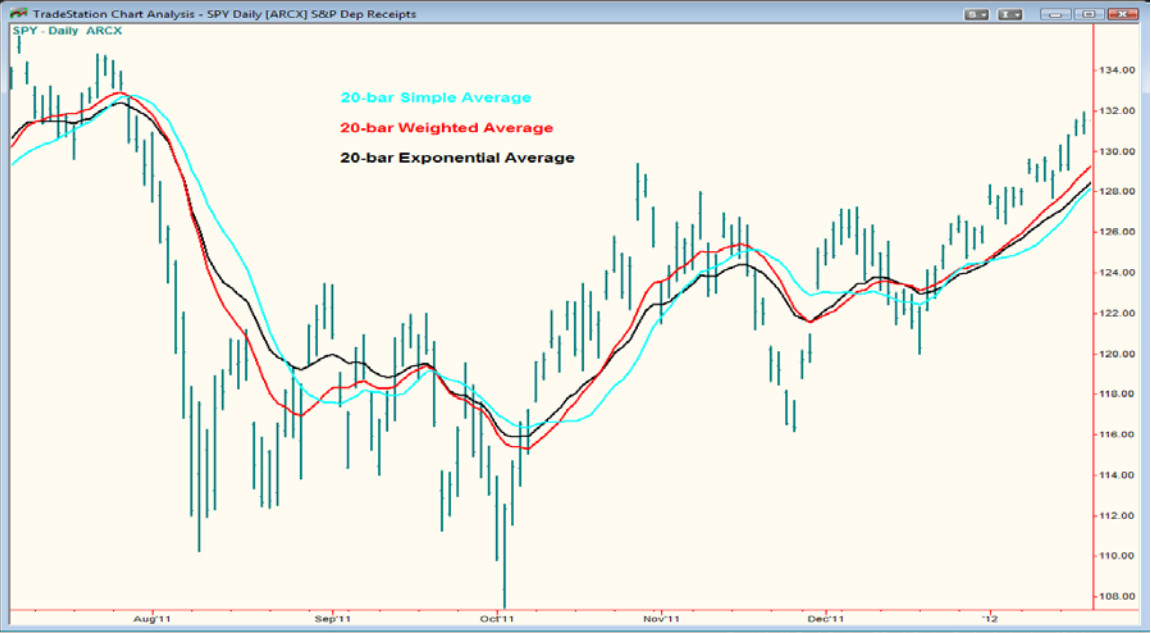
\includegraphics[width=\textwidth]{background/movingaverages}
    \caption{Simple Moving Average (MA) [blue], Weighted MA [red] and Exponential MA of the S\&P500 \protect\footnotemark \parencite[Fig. 5]{dash2012movingaverages}}
    \label{fig:dashweightedaverages}
\end{figure}
\footnotetext{A stock market index of 500 American companies, the US equivalent of the FTSE 500}

These techniques can be applied to a discrete set of numerical time series data, such as personal expenditure over time in order to make an estimate of what the next value in the series will be \parencite{filliben2003nist}. A prediction can be made using the formula in Fig. \ref{fig:weightedmeanforumla}, where $w_{i}$ is the weight and $x_i$ is the value at time period $i$. Simple smoothing is the equivalent of $w_i = 1$, while exponential smoothing is based around a negative exponential law such as $w_i = \exp(-n+i)$, both are examples of weighted smoothing and the weights can be decided in different ways depending on what is being predicted. Time periods with a higher weight have a greater affect on the mean, so in order to make a future prediction, the most recent time period would have a higher weight. \question{The chosen implementation details in the design section}

\begin{figure}[h]
    \centering
    \[
        \frac{w_1 x_1 + w_2 x_2 + \cdots + w_n x_n}{w_1 + w_2 + \cdots + w_n}.
    \]
    \caption{Using weighted smoothing to predict a future value}
    \label{fig:weightedmeanforumla}
\end{figure}

% Holt winters extends smoothing, to take into account trends in data
Smoothing (and therefore prediction) can be extended to take into account trends and possible seasonal fluctiations using double and triple smoothing, respectively. A technique known as `Holt-Winters double exponential smoothing` takes into account trends in data, which single smoothing does perform accurately with, by factoring the smoothed average growth between previous time series when calculating the average for each period \parencite{kalekar2004holtwinters}. \question{A demonstration of this is in chapter X?}

% 
Extending the calculation into double and triple smoothing when estimating a users future outflow was decided as a possible extension for the project. \question{Where to mention this?} 

\section{Security}
\question{Should I mention the password entropy paper here? Currently in implementation}


